%% Research proposal: a signal-loss audit of network filters for the Turkish GNSS network.
%% Draft for the author to read and rework into a TÜBİTAK application. Not for submission as is.
\documentclass[preprint,12pt,authoryear]{elsarticle}

\usepackage[T1]{fontenc}
\usepackage[utf8]{inputenc}
\usepackage{lmodern}
\usepackage{amsmath,amssymb}
\usepackage{booktabs}
\usepackage{array}
\usepackage{graphicx}
\usepackage{xcolor}
\usepackage{microtype}
\usepackage{tikz}
\usetikzlibrary{positioning,arrows.meta}
\usepackage[hidelinks]{hyperref}

\setlength{\emergencystretch}{2em}

\journal{research proposal, draft}

\begin{document}

\begin{frontmatter}

  \title{Noise Removal versus Signal Loss in Network Filtering of Daily GNSS Time Series: A Signal-Loss Audit on the Turkish Network}

  \author{H. O\u{g}uz Bolat}
  \ead{oguz.bolat@std.yildiz.edu.tr}
  \affiliation{organization={Department of Geomatics Engineering, Y{\i}ld{\i}z Technical University},
    city={Istanbul},
  country={T\"urkiye}}

  \begin{abstract}
    Network filters remove the common-mode error of GNSS position time series by predicting each station from other stations and subtracting the prediction. Every such filter also removes whatever real deformation the other stations share with the target, and the published evaluations of these filters, which rest on the reduction of residual scatter, cannot see this loss. This project proposes a signal-loss audit of network filters on the daily solutions of the continuously operating GNSS stations of T\"urkiye, as published by the Nevada Geodetic Laboratory. Transients of known extent, amplitude and duration are planted in the real residuals of the network; each filter is run with and without them; and the paired difference gives the fraction of each transient that survives, together with the noise the filter removes, the spurious signal it creates elsewhere, and the fraction of each station's seasonal cycle, of real earthquake offsets and of real postseismic deformation that it keeps. Classical target-inclusive filters, distance-excluded stacks, leave-one-out filters over nearest neighbours and learned filters, including attention networks, are audited under one protocol in which the exclusion radius around the target and the number of stations read are experimental variables. The Turkish network, with a median station spacing of about 60~km, is the sparse counterpart of the dense networks on which these filters have been developed, and the audit will state, for the first time with ground truth, what each filter costs in signal on such a network and which filter settings keep the deformation signals that studies of the Anatolian fault systems depend on. The method was developed and tested on 1,251 stations in California; the Turkish data set is held out, with its test period untouched until the method is frozen.
  \end{abstract}

  \begin{keyword}
    GNSS time series \sep common-mode error \sep spatial filtering \sep transient deformation \sep signal preservation \sep deep learning \sep T\"urkiye
  \end{keyword}

\end{frontmatter}

\noindent\fbox{\parbox{0.97\textwidth}{\small Status of this document. This is a draft research proposal, written on 5 November 2026 for the author to read and rework into a project application. Its text was drafted by Claude Fable 5.1 (Anthropic) through Claude Code, at the author's request, from the repository, its design documents, the internal working report on the California development work and the coverage analysis of the Turkish data. The research questions are the author's. Statements about the Turkish data were measured on the downloaded series on 5 November 2026; statements about the California development work describe results obtained with a processing in which the seasonal cycle was removed, which the author has since reversed, so those results are indicative only and are cited without numbers. Nothing in this document has been computed on the Turkish test period.}}

%% ===========================================================================
\section{Summary}
\label{sec:summary}
%% ===========================================================================

Continuously operating GNSS stations record crustal deformation together with noise, part of which is common to many stations of a network. Network filters estimate this common-mode error from the other stations and subtract it, and are a standard step before the detection of transient deformation, the estimation of velocities and the study of postseismic processes. The literature evaluates these filters almost exclusively by the reduction in the scatter of the filtered series. Scatter reduction, however, rewards the removal of anything the stations share, deformation included, and no study has measured with ground truth how much real signal a filter removes as a function of the signal's size relative to the filter's reach.

The project will carry out such a measurement on the Turkish network. Its aims are (i) to quantify, for each filter family, the fraction of a transient that survives filtering as a function of the transient's width, amplitude and duration and of the filter's exclusion radius and number of stations; (ii) to measure, on the same runs, the noise removed, the spurious signal created elsewhere, the fraction of each station's seasonal cycle kept, and the retention of real earthquake offsets and real postseismic deformation; (iii) to compare classical, distance-excluded, leave-one-out and learned filters at equal signal kept rather than on noise alone; and (iv) to deliver, as open software, an audit that any future filter for the Turkish network can be run through.

The data are the daily positions of the Turkish continuously operating stations as published by the Nevada Geodetic Laboratory, which cover the network densely from 2009 to October 2015, and again in September to December 2020 and from September 2022 to April 2023. These windows contain the 2011 Van (M 7.1), 2014 G\"ok\c{c}eada (M 6.9), 2020 Samos (M 7.0) and 2023 Kahramanmara\c{s} (M 7.8 and 7.5) earthquakes, which provide the real-signal checks. The method, the software and the protocol exist and were developed on 1,251 stations in California; the Turkish data set is the held-out network on which they will be applied once, under a protocol in which the test period is not examined until the method is frozen.

%% ===========================================================================
\section{Background and significance}
\label{sec:background}
%% ===========================================================================

\subsection{Common-mode error and its removal}

Daily GNSS position time series contain, besides the deformation of the ground, noise that is correlated across a network: errors in satellite orbits and clocks, in the realisation of the reference frame and in the modelling of large-scale environmental loading \citep{wdowinski1997, dong2006, kreemer2021}. This common-mode error has been estimated by stacking the residuals of the other stations \citep{wdowinski1997}, by principal or independent component analysis \citep{dong2006, gruszczynski2018, zhou2022}, and by weighted means and medians of neighbouring stations \citep{tianshen2016, kreemer2021}. Network filtering began with the Southern California Integrated GPS Network, where the common mode was the weighted mean of the residuals of the other stations \citep{wdowinski1997}; principal component analysis and the Karhunen--Lo\`eve expansion extended this to common modes that vary in space \citep{dong2006}; and later work made principal component filtering applicable to networks whose stations start and stop at different times \citep{shen2014, gruszczynski2018, li2020vbpca}. Because the common mode varies in space, large networks have been divided into sub-regions \citep{liu2026}. \citet{tianshen2016} weighted each neighbouring station by its distance and by the correlation of its residuals with the target and chose the weights by minimising the residual scatter after filtering; \citet{kreemer2021} take a correlation-weighted median over nearby stations, the target included when it qualifies. Across this family, performance is reported as scatter reduction, reduced inter-station correlation, velocity uncertainty or the recovery of a simulated common mode. \citet{kreemer2021} themselves note that the main reason their filter reduces scatter more than traditional stacking is that it absorbs local common-mode transients.

\subsection{Learned filters}

Deep learning has entered the field from two sides. The graph neural network of \citet{bachelot2025} predicts each station from its eight nearest stations beyond 400~km; the distance was chosen empirically, in Cascadia, as the shortest at which 280 observed slow-slip offsets were no longer reduced by denoising, and a plain stack of the same distant stations performed comparably. \citet{costantino2024} train graph recurrent layers and transformers to extract slow slip from synthetic examples added to noise synthesised from real series, and later used the denoised data to invert fifteen years of slow slip \citep{costantino2026}. \citet{mastella2025} model high-frequency scatter at single stations with synthetic training noise. \citet{teutschmann2026} pretrained a self-supervised model on 17,651 stations of the Nevada Geodetic Laboratory. Predicting a withheld sensor from its neighbours is an established principle elsewhere, in ocean-bottom seismology \citep{crawfordwebb2000, janiszewski2019}, distributed acoustic sensing \citep{batson2019, vandenende2023} and spatiotemporal kriging \citep{wu2021ignnk, cini2022grin, marisca2022spin}, and excluding nearby observations so that spatial autocorrelation does not inflate apparent skill is the basis of buffered spatial cross-validation \citep{lerest2014}.

\subsection{How signal preservation has been assessed}

Three approaches recur. Observed transients can be compared before and after filtering \citep{bachelot2025}; this uses real signals but has no ground truth. Synthetic signals can be added to synthetic noise \citep{costantino2024, mastella2025}; this has ground truth but depends on how realistic the noise is, and has been analysed against signal-to-noise ratio rather than spatial scale. Independent data, such as tectonic tremor, can confirm that an extracted signal is real \citep{costantino2024}, but cannot measure what was lost. In Cascadia, \citet{costantino2026} report that the scaling, b-value and stress-drop distribution of slow-slip events change with the detection threshold applied to slip inverted from denoised data, and the debate over a reported precursory acceleration of slip before large earthquakes \citep{bletery2023, bletery2025} turned on whether a common-mode correction removes only noise. The question of what a filter removes is therefore not a technicality: it decides which published deformation signals are real.

\subsection{Gaps}

Four gaps motivate the project. No study has measured, with ground truth, how much of a transient a common-mode filter removes as a function of the transient's size relative to the filter's reach. The reach has been chosen empirically, as a fixed 400~km \citep{bachelot2025} or by scatter-based thresholds \citep{tianshen2016}. Filters that use the target station, which include most classical methods, have not been compared with leave-one-out filters on signal loss. And learned filters have been compared with simple ones on noise reduction, not at equal signal kept. A fifth gap is specific to this project: every filter in this literature was developed and evaluated on dense networks, in California, Cascadia, Japan or western Europe, with station spacings of ten to thirty kilometres. The Turkish network, with a median spacing of about 60~km, is representative of the national networks of most countries, and no signal-loss result exists for a network of this kind.

\subsection{Significance for T\"urkiye}

The Anatolian fault systems produce the deformation signals that network filters are most likely to damage: afterslip and postseismic relaxation that extend over hundreds of kilometres after the 1999 \.{I}zmit, 2011 Van, 2020 Samos and 2023 Kahramanmara\c{s} earthquakes, and the slow strain accumulation along the North and East Anatolian faults. Every study of these processes from GNSS data filters the series first. An audit that states, for each filter and setting, what fraction of a transient of a given size survives, and how far from a real event a filter's spurious signal reaches, gives those studies a quantitative basis for their choice of filter, and gives the operators of the national network a tool to evaluate any processing they adopt. The project also delivers the first systematic application of learned filters to Turkish GNSS data, under a protocol that measures their cost in signal rather than their gain in scatter alone.

%% ===========================================================================
\section{Aims and research questions}
\label{sec:aims}
%% ===========================================================================

The project tests one hypothesis and answers four questions.

\paragraph{Hypothesis} The fraction of a transient that a network filter removes is set by the share of the filter's input that lies inside the transient: a filter over the nearest stations removes most of any transient wider than their spacing, while a filter over the whole network loses only the share of the transient that enters the network mean, which reappears with opposite sign at every other station.

\paragraph{Questions}
\begin{enumerate}
  \item For each filter family, how does the retention of a planted transient depend on its width, amplitude and duration, and on the filter's exclusion radius and number of stations, on a network with a 60-km spacing?
  \item At equal signal kept, which filter removes most noise, and does any learned filter remove more than the unweighted mean of all distant stations?
  \item How much of a station's seasonal cycle, of real coseismic offsets and of real postseismic deformation does each filter keep, and how far does the spurious signal of a real event reach through each filter?
  \item Do the answers obtained on a dense network (California, where the method was developed) transfer to the sparse Turkish network, or does the trade-off between noise removed and signal kept shift with station spacing?
\end{enumerate}

%% ===========================================================================
\section{Data}
\label{sec:data}
%% ===========================================================================

\subsection{The Turkish stations in the Nevada Geodetic Laboratory archive}

The data are the daily IGS20 solutions of the Nevada Geodetic Laboratory (NGL) \citep{blewitt2018, ngl2026}, which processes the public RINEX files of continuously operating stations worldwide with one software and one reference frame. Each solution gives the east, north and up position of a station's antenna relative to a fixed reference point near the station, estimated from 24 hours of observations, with formal uncertainties of about 1~mm in the horizontal and 3--4~mm in the vertical. Using the NGL archive rather than an in-house processing has two advantages for an audit: every station is processed identically, and the filters audited here are the filters that users of this public archive apply.

All NGL stations between $35.5^\circ$ and $42.5^\circ$N and between $25.5^\circ$ and $45.0^\circ$E were examined on 5 November 2026: 312 stations, of which most belong to the national continuously operating network (TUSAGA-Aktif) and the remainder to international and research networks. The archive's station table reports long spans for these stations, but the daily series themselves show that the national network is present only in three windows (Table~\ref{tab:coverage}): from 2009 to October 2015, with 110--165 stations reporting on a typical day; from September to December 2020, with 90--140; and from September 2022 to April 2023, with 150--160. Outside these windows 10--35 stations report. The raw observations of the national network for the other years are not publicly available, and the project does not depend on obtaining them.

\begin{table}[tbp]
  \centering
  \caption{Stations of the Turkish box reporting daily solutions in the NGL archive, by period (measured on the downloaded series, 5 November 2026), and the earthquakes of M $\ge$ 6.5 catalogued at them.}
  \label{tab:coverage}
  \small
  \begin{tabular}{l r l}
    \toprule
    Period & Stations reporting & Earthquakes (stations with a catalogued step) \\
    \midrule
    2009 -- Oct 2015 & 110--165 & 2010 Elaz{\i}\u{g} M 6.1 (17); 2011 Van M 7.1 (58); 2014 G\"ok\c{c}eada M 6.9 (45) \\
    Nov 2015 -- Aug 2020 & 15--30 & 2017 Bodrum--Kos M 6.6 (19); 2020 Elaz{\i}\u{g} M 6.7 (25) \\
    Sep -- Dec 2020 & 90--140 & 2020 Samos M 7.0 (59) \\
    2021 -- Aug 2022 & 12--30 & 2022 D\"uzce M 6.1 (19, November 2022) \\
    Sep 2022 -- Apr 2023 & 150--160 & 2023 Kahramanmara\c{s} M 7.8 (174) and M 7.5 (159); 2023 Hatay M 6.3 (12) \\
    May 2023 -- 2026 & 10--35 & -- \\
    \bottomrule
  \end{tabular}
\end{table}

In the first window, 159 stations have at least 1,200 daily solutions, with a mean coverage of 0.79--0.91 per year. Their median distance to the nearest station is 62.7~km (quartiles 53.5 and 70.1~km), a typical station has no other station within 50~km and four within 100~km, and the network spans $35.5$--$42.4^\circ$N and $25.6$--$45.0^\circ$E. For comparison, the Californian network on which the method was developed has a median nearest-neighbour distance of 9.7~km and a typical station has 22 stations within 50~km. Of the stations of the 2020 and 2022--2023 windows, 78 and 79 respectively are among the 159 stations of the first window.

\subsection{Consequences for the design}

The data impose the design of the study. The first window, 6.7 years long, is the development data set: filters are tuned and learned filters trained on its first years, with the later years for validation and test. The two later windows, four and eight months long, are too short to train on but each contains a major earthquake with offsets at most of the network and several months of postseismic motion, so they serve as held-out real-signal tests to which the filters frozen on the first window are transferred. Within the first window, the 2011 Van earthquake and its postseismic deformation are excluded from training and scored separately, as the 2019 Ridgecrest earthquake was in the Californian development, and the 2014 G\"ok\c{c}eada earthquake falls in the validation years. The project therefore has four real-signal tests at four different places and times, two of them never seen during development.

The 60-km spacing changes what the audit can and cannot resolve. A transient 10 or 25~km wide covers at most one station, so no filter built from other stations can remove it and no filter can be evaluated on it; the informative widths on this network are 50--300~km, and the exclusion radii 0--400~km. Learned filters that read many neighbours will read stations that are farther away than in California, and the number of station-days available for training is about twenty times smaller than there. These are not weaknesses of the design but the conditions under which filters are actually applied to national networks, and question 4 of Section~\ref{sec:aims} is about exactly this shift.

%% ===========================================================================
\section{Method}
\label{sec:method}
%% ===========================================================================

The method is implemented in the open \texttt{gnssdl} package, written and tested during the Californian development (148 automated tests, including the leak checks of Section~\ref{sec:loo}). Figure~\ref{fig:pipeline} shows the processing chain: daily positions are reduced to residuals by removing each station's trajectory, screened, and stored in a single array; every filter is applied to this array; and the cleaned series are scored by the audit.

\begin{figure}[tbp]
  \centering
  \resizebox{\textwidth}{!}{%
    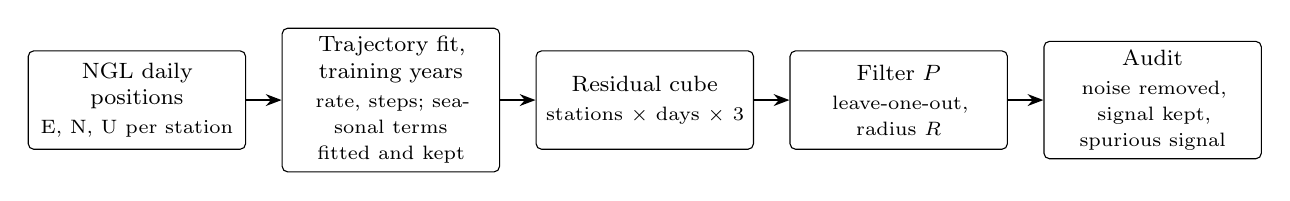
\begin{tikzpicture}[
        box/.style={draw, rounded corners=2pt, align=center, font=\footnotesize, minimum height=1.25cm, text width=2.55cm, inner sep=3pt},
        arr/.style={-{Stealth[length=2mm]}, thick},
      node distance=0.45cm]
      \node[box] (raw) {NGL daily positions\\[1pt]{\scriptsize E, N, U per station}};
      \node[box, right=of raw] (traj) {Trajectory fit, training years\\[1pt]{\scriptsize rate, steps; seasonal terms fitted and kept}};
      \node[box, right=of traj] (res) {Residual cube\\[1pt]{\scriptsize stations $\times$ days $\times$ 3}};
      \node[box, right=of res] (filt) {Filter $P$\\[1pt]{\scriptsize leave-one-out, radius $R$}};
      \node[box, right=of filt] (score) {Audit\\[1pt]{\scriptsize noise removed, signal kept, spurious signal}};
      \draw[arr] (raw) -- (traj);
      \draw[arr] (traj) -- (res);
      \draw[arr] (res) -- (filt);
      \draw[arr] (filt) -- (score);
    \end{tikzpicture}}
  \caption{Processing chain. Planted transients are added to the residual cube before filtering, and the paired difference of the cleaned series gives the fraction kept.}
  \label{fig:pipeline}
\end{figure}

\subsection{Residuals}
\label{sec:residuals}

For each station $i$ and component $c$, the trajectory model
\begin{equation}
  x_{i,c}(t) = a + v\,(t - t_0) + \sum_{k=1}^{2}\left[p_k \sin(2\pi k t) + q_k \cos(2\pi k t)\right] + \sum_{j} b_j\, H(t - t_j) + r_{i,c}(t)
  \label{eq:trajectory}
\end{equation}
is fitted by least squares on the training years, where $a$ is a constant, $v$ a linear rate about the mean epoch $t_0$ of the fitted data, $p_k$ and $q_k$ the amplitudes of the annual and semi-annual harmonics, $b_j$ the amplitudes of Heaviside steps $H$ at the epochs $t_j$ of the NGL step catalogue and $t$ the time in years. The fitted trajectory is extrapolated to the later years. The residual $r_{i,c}(t)$ is the series minus the constant, the rate and the equipment steps. The seasonal terms are estimated so that an incomplete cycle does not bias the rate, but they are added back: the residual carries each station's seasonal cycle, and what a filter does to it is measured directly (Section~\ref{sec:measures}). Earthquake steps are likewise estimated and added back, so that coseismic offsets, which are spatially coherent deformation of the kind a filter should preserve, remain in the series. Equipment steps are removed everywhere, within the training years in the fit and after them by a local estimate, the median residual over the 30 days after the change minus that over the 30 days before. A value more than five robust standard deviations from its 61-day running median is treated as missing. A station is dropped if the robust scale of a second fit, from which earthquake steps are also removed, exceeds 10~mm in the horizontal or 30~mm in the vertical, which removes non-tectonic site motion; and stations within 1~km of a longer-running station are dropped as duplicates. The residuals, their uncertainties and an availability mask are stored with the neighbour lists of every station at each exclusion radius.

\subsection{Leave-one-out filtering and the exclusion radius}
\label{sec:loo}

A filter $P$ estimates the part of the residual of station $i$ that is shared with other stations, and the cleaned series is $r - P(r)$. A leave-one-out filter never reads station $i$ itself when estimating it, and never reads any station within $R$~km of it. The exclusion radius $R$ and the number of stations read are experimental variables, run at $R = 0$, 50, 100, 200 and 400~km for the filters over the whole network and at $R = 0$, 50, 100, 200 and 400~km for those over nearest neighbours; the final radii are fixed on the validation years before the test period is touched. Target-inclusive filters, which read the target on purpose as published filters of their kind do, are applied to the same data and scored on noise removed and on the signal measures, but not on reconstruction error.

Two leak checks are run for every leave-one-out filter at every radius. In the radius check, the target and every station within $R$ of it are set to a poison value of $10^6$~mm, for five randomly chosen targets; in the mask check, cells hidden from a filter are filled once with missing values and once with the poison value. In both, the predictions must agree to within 0.001~mm. A filter that passes never reads what it must not, and one prediction on the unhidden data is then a leave-one-out prediction for every station at once.

\subsection{Measures}
\label{sec:measures}

Filters are compared on two measures of noise and five of signal, all computed from the same runs; the planted transients are the primary signal test, and the real signals are secondary checks without ground truth.

\emph{Noise removed} is the reduction in short-period scatter at each scored station, $1 - \mathrm{rms}(\mathrm{fast}(r - P(r))) / \mathrm{rms}(\mathrm{fast}(r))$, where the fast part of a series is the series minus its 61-day running median; it is averaged over the three components and summarised by its median over stations. Predicting zero gives 0. The measure covers periods shorter than about two months.

\emph{Reconstruction error} is the root mean square of the fast part of the leave-one-out error $r - P(r)$, in units of each station's robust noise scale. It is the criterion on which the leave-one-out filters are tuned, on the validation years. Because the error is lower when the prediction reproduces whatever the target shares with other stations, signal included, tuning on it favours settings that absorb coherent signal; the signal measures are therefore independent checks on what the tuning selected, not refinements of it.

\emph{Retention} measures the fraction of a planted transient that survives filtering. A transient $s$ is added to the residuals, both the original and the modified residuals are filtered, and the change in the cleaned series and the retention are
\begin{equation}
  \Delta = \big(r + s - P(r+s)\big) - \big(r - P(r)\big),
  \qquad
  \rho = \frac{\langle \Delta,\, s \rangle}{\langle s,\, s \rangle},
  \label{eq:retention}
\end{equation}
with the inner products over the horizontal components, the days of the transient and the scored stations within twice its width of its centre. Pairing with the unmodified run removes the noise term; for a linear filter, $\rho = \langle s - P(s), s\rangle / \langle s, s \rangle$ exactly. $\rho = 1$ means that the transient is kept, $\rho = 0$ that it is removed, and $\rho > 1$ that the filter adds to it.

\emph{Spurious signal} is the change $\Delta$ created at scored stations outside the transient's footprint, reported as the largest peak horizontal amplitude in units of the planted amplitude, together with the number of stations affected and the sum of their peak changes, since a network-wide filter spreads a small ghost over every station while a local filter creates a larger one at a few.

\emph{Seasonal kept} fits, per scored station and component over the period, constant, rate, annual and semi-annual terms and Heaviside steps at the station's catalogued earthquakes to $r$ and to $r - P(r)$ on the same days, and reports $\langle c_{\mathrm{kept}}, c_{\mathrm{obs}} \rangle / \langle c_{\mathrm{obs}}, c_{\mathrm{obs}} \rangle$ over the four harmonic coefficients $c$. A station's seasonal cycle is nearly the same across a network, so it is the limiting case of a wide transient; a filter that averages the network is expected to remove most of it, and the measure states how much of each station's own cycle survives.

\emph{Real offsets} are every catalogued earthquake step in the scored period at a scored station with an observed horizontal offset of at least 3~mm and no other step within 15 days; the offset is the mean position over the 10 days after the earthquake minus that over the 10 days before, and the fraction kept is the same projection computed on the cleaned series.

\emph{Real postseismic deformation} is scored at the stations within 150~km of a chosen earthquake as the horizontal displacement over days 7--365 after the mainshock, relative to the mean of days 1--6, projected on the same quantity in the cleaned series. The interval is excluded from training.

\subsection{Planted and real signals}
\label{sec:planted}

Gaussian transients have the form $s(d, t) = A \exp(-d^2 / 2L^2)\, g(t)\, \mathbf{u}$, where $d$ is the distance of a station from the centre, $A$ the amplitude, $L$ the width, $\mathbf{u}$ a horizontal unit vector in a random direction and $g(t)$ a raised-cosine rise over $D$ days, a 60-day hold and a raised-cosine fall, so the transient leaves no permanent offset. The grid is $A \in \{2, 5, 10\}$~mm, $D \in \{10, 30, 90\}$~days and, for the Turkish spacing, $L \in \{50, 100, 200, 300\}$~km, each combination planted at 20 centres chosen among the scored stations, with many transients sharing one run of a filter where no station can be changed by two of them.

The audit's signal tests are these planted transients. A library of realistic fault-slip events, built in the Californian development from published source models placed on catalogued faults, is not used in this project; it may be added later for the Anatolian faults, and the software supports it.

Real signals are the 2011 Van earthquake (excluded from training, scored as postseismic deformation and offsets), the 2014 G\"ok\c{c}eada earthquake in the validation years (offsets), and the 2020 Samos and 2023 Kahramanmara\c{s} earthquakes in the held-out windows (offsets and postseismic deformation). These observed signals have no ground truth, since the observed offset includes noise, and complement the planted ones.

\subsection{Filters}
\label{sec:filters}

Table~\ref{tab:filters} lists the filters. C1 is the stack of \citet{wdowinski1997}; C3 is sub-regional probabilistic principal component analysis \citep{tipping1999, gruszczynski2018, liu2026} with 1, 2 or 4 regions and 1--3 components; M2-self is the robust weighted median with the target included, as in common-mode component imaging \citep{tianshen2016, kreemer2021}. The far stack is the unweighted mean of every station beyond $R$, the target excluded, and is the parameter-free baseline; D1 is the far stack at 400~km, the distance of \citet{bachelot2025}. M1 is the distance-weighted mean of the nearest stations, M2 its robust weighted median after outlier screening \citep{kreemer2021}, M3 ridge regression on the neighbours' components per station or pooled, and M4 the same per period band. The learned filters are M3k, a kernel whose neighbour weights are learned from distance, azimuth and noise level but never from the values; M5, a space--time attention network that predicts a correction to the far stack from the target's neighbours and the far stack over a 64-day window; and M6, an attention network over a wider set of stations or the whole network, in which geometry enters only as a learned bias from pairwise distance and azimuth. Each learned filter is also trained with planted transients in its inputs but not in its targets (the ``-aug'' versions), which in the Californian development was the training that stopped the network from absorbing coherent signal. Learned filters are trained on quiet residuals, the residuals minus the earthquake offsets estimated in the fit, on training days outside the Van exclusion and outside $\pm 30$ days of M $\ge$ 6 earthquakes, with early stopping on the validation reconstruction error and three training seeds. The number of neighbours for the nearest-neighbour filters will be 8, 16 and 32, since 16 nearest stations on this network already reach about 200~km.

\begin{table}[tbp]
  \centering
  \footnotesize
  \caption{Filter configurations to be audited. Stations read: the other stations a prediction for the target uses; ``nearest'' means the nearest stations beyond $R$. Days used: days of other stations read by a prediction for day $t$.}
  \label{tab:filters}
  \setlength{\tabcolsep}{4pt}
  \begin{tabular}{l >{\raggedright\arraybackslash}p{5.2cm} >{\raggedright\arraybackslash}p{2.6cm} l}
    \toprule
    Name & Description & Stations read & Days used \\
    \midrule
    \multicolumn{4}{l}{\textit{Target-inclusive}} \\
    C1 & Unweighted mean of the whole network & All + target & $t$ \\
    C3 & Sub-regional probabilistic PCA, several settings & Region + target & $t$ \\
    M2-self & Robust weighted median of the neighbours and the target & Nearest + target & $t$ (31 d) \\
    \multicolumn{4}{l}{\textit{Distance-excluded}} \\
    Far stack & Unweighted mean of every station beyond $R$ & All beyond $R$ & $t$ \\
    D1 & Far stack at $R = 400$~km & All beyond 400~km & $t$ \\
    \multicolumn{4}{l}{\textit{Leave-one-out over nearest neighbours}} \\
    M1 & Distance-weighted mean & 8, 16, 32 nearest & $t$ \\
    M2 & Robust weighted median after outlier screening & Nearest & $t$ (31 d) \\
    M3a, M3b & Ridge regression per station, and pooled with neighbour geometry & Nearest & $t$ \\
    M4a, M4b & M3 per period band & Nearest & All \\
    \multicolumn{4}{l}{\textit{Learned}} \\
    M3k & Learned kernel from distance, azimuth and noise level & Nearest & $t$ \\
    M5, M5-aug & Space--time attention, correction to the far stack & Nearest + far stack & 64 d \\
    M6, M6-aug & Attention over many stations or the whole network, with and without the far-stack correction & $N$ nearest or all & 64 d \\
    \bottomrule
  \end{tabular}
\end{table}

\subsection{Protocol}
\label{sec:protocol}

The days of the first window are split into training (2009--2012), validation (2013--2014) and test (January to October 2015) years; the 2020 and 2022--2023 windows are held-out blocks. Ten percent of the stations are held out by farthest-point sampling \citep{gonzalez1985} and never used in training, so that the generalisation of learned filters to unseen stations is measured. All design decisions, tuning and model selection are made on the validation years. The method is then frozen, with a tagged version of the software, and the test year and the held-out blocks are scored once, with the settings chosen on validation; no result from them is examined before the freeze, and the project's statements about them are made from that single scoring. Differences between filters are tested with a paired block bootstrap over stations and 30-day blocks for reconstruction error, and by resampling the planted transients, paired by identifier, for retention; a difference whose interval includes zero is reported as not distinguishable. A filter is reported as better than the far stack only if its error is lower with an interval excluding zero and its retention of wide transients and its spurious signal are within 0.05 of the far stack's; a filter that fails the signal conditions is reported as a noise gain bought with signal, whatever its error.

%% ===========================================================================
\section{Preliminary work}
\label{sec:preliminary}
%% ===========================================================================

The method, the software and the protocol were developed between October and November 2026 on the NGL daily solutions of 1,251 stations in and around California, with seventeen filter configurations from the four families above. That development established the audit's measures, the leak checks, the planted-transient tests, the real-offset and postseismic tests and the bootstrap comparisons, and it produced three findings that shape this proposal. First, the retention of a planted transient by the mean of all stations matched, within a few hundredths, the share of stations the transient covers, computed from the station positions alone; and filters over the 16 nearest stations removed most of any transient wider than their spacing. Second, no learned filter reduced the reconstruction error below that of the far stack with an interval excluding zero, and every learned filter trained without planted transients kept less signal than the far stack; training with planted transients in the inputs brought the attention networks' retention up to, not beyond, the far stack's. Third, scatter reduction and reconstruction error rewarded filters that absorbed signal or the target's own noise, so a comparison of filters that omits signal kept and spurious signal can rank a filter that removes signal above one that does not. These results were obtained with a processing that removed the seasonal cycle before filtering, which has since been reversed in favour of keeping it and measuring it; they are therefore cited here as the development evidence for the design, without their numbers, and the Californian data set is development data only. The Turkish data set has been downloaded and its coverage measured (Section~\ref{sec:data}); nothing has been filtered or scored on it.

%% ===========================================================================
\section{Work plan}
\label{sec:workplan}
%% ===========================================================================

\begin{enumerate}
  \item \emph{Data and processing (months 1--2).} Build the residual cube of the 2009--2015 window and of the two held-out windows with the processing of Section~\ref{sec:residuals}; review the dropped stations; fix the training, validation and test years and the held-out stations.
  \item \emph{Reference and leave-one-out filters (months 2--4).} Run the target-inclusive, distance-excluded and nearest-neighbour filters at every radius on the validation years; tune their settings; run the leak checks.
  \item \emph{Learned filters (months 4--8).} Train the learned kernel and the attention networks, with and without planted transients, at every radius and with three seeds; select on validation reconstruction error; examine the sensitivity of training to the smaller number of station-days.
  \item \emph{Signal tests on validation (months 6--9).} Planted transients, seasonal kept, the G\"ok\c{c}eada offsets and the Van postseismic test for every filter and radius; the trade-off between noise removed and signal kept; comparison with the Californian development results (question 4).
  \item \emph{Freeze and held-out scoring (month 10).} Freeze the method and software; score the test year and the 2020 and 2022--2023 windows once; the Samos and Kahramanmara\c{s} offsets and postseismic deformation.
  \item \emph{Reporting (months 10--12).} Manuscript, open release of the software, the episode and event lists, the results tables and the trained models.
\end{enumerate}

%% ===========================================================================
\section{Expected outcomes}
\label{sec:outcomes}
%% ===========================================================================

The project will deliver: (i) retention, spurious signal and noise removed as functions of transient width and exclusion radius for every filter family on the Turkish network, with bootstrap intervals; (ii) the fraction of each station's seasonal cycle, of the Van, G\"ok\c{c}eada, Samos and Kahramanmara\c{s} offsets and of the Van and Kahramanmara\c{s} postseismic deformation kept by each filter, the last two measured on data never seen during development; (iii) a comparison of learned and classical filters at equal signal kept, and a statement of whether any learned filter beats the mean of all distant stations on this network; (iv) a direct comparison of the trade-off between a dense and a sparse network, since the same software and measures were applied to both; (v) a recommended filter and exclusion radius for studies of transient deformation on the Turkish network, stated with the signal cost of the alternatives; and (vi) the open \texttt{gnssdl} package, through which any future filter or processing of the national network can be audited with the same protocol.

%% ===========================================================================
\section{Risks and limitations}
\label{sec:risks}
%% ===========================================================================

The development data set is 6.7 years long and about 290,000 station-days, against twelve years and several million station-days in California; the attention networks may not train to the same point, and the project will report their training behaviour and, if needed, their smaller variants as a result in its own right rather than a failure. The test year is ten months long, so its statistical power is lower than that of the held-out windows, and the project's strongest held-out statements will come from the 2020 and 2022--2023 blocks. Only 78--79 of the stations of those blocks were present in 2009--2015, so per-station filters (M3a, M4a) transfer to them only partly; pooled and learned filters transfer fully. The quality of the national network's daily solutions in the NGL archive has not been examined before; the station quality control of Section~\ref{sec:residuals} will drop unstable sites, and the dropped list will be published. The planted transients are Gaussian in space and symmetric in direction, and do not reproduce the two-sided displacement field of fault slip; the realistic event library is left for later work. The real signals have no ground truth. Noise removed is a fast-band measure, and the long-period common mode is reached only through the seasonal and postseismic measures. The 60-km spacing means that transients narrower than about 50~km cannot be evaluated on this network; the audit states this as a property of the network rather than of the filters.

%% ===========================================================================
\section{Data, code and use of AI tools}
\label{sec:availability}
%% ===========================================================================

The daily solutions are publicly available from the Nevada Geodetic Laboratory \citep{ngl2026}. The \texttt{gnssdl} package is openly available at \url{https://github.com/hogib/gnssdl} under the MIT licence, with its tests, design documents and the figure code; the results tables, trained models, planted-signal catalogues and the frozen version of the software will be released with the manuscript. The software, its tests and this proposal's text were written by Claude (Anthropic) through Claude Code under the author's direction; the research questions, the design decisions and the choice of study area are the author's.

\bibliographystyle{elsarticle-harv}
\bibliography{../../paper/references}

\end{document}
